\scanpage{99}\mspage{95}
Il reste seulement à prouver que si $\alpha_{*}$ est dans $\operatorname{Corr}(\Sigma,\Sigma')$, alors $\alpha=\varphi(\alpha_{\unsure{\times|*}})$ satisfait aux conditions de \unsure{propo|prop.} 4\unsure{,} et \unsure{redonne} $\alpha_{*}$, par
\[
 \alpha_{*}(S)=\mathop{\mathrm{Sup}}\limits_{x\in S}{}_{\Sigma_{E'}}
 \underset{\inserted{\substack{\Vert\,\text{\unsure{def.|déf.}}\\
 \alpha_{*}^{\unsure{\cdot|\prime}}(\operatorname{supp}^{\unsure{\bullet|\circ}}_E(x))}}}{\underline{\alpha(x)}}
 \qquad(S\in\Sigma_E)\unsure{,|.}
\]
\deleted{Ce qui}\inserted{Cette formule} provient de la formule
\[
 S=\mathop{\mathrm{Sup}}\limits_{x\in S}{\unsure{\operatorname{supp}|\deleted{\operatorname{supp}}\sigma}}^{\bullet}_E(x)
\]
et de la commutation de $\alpha_{*}$ avec $\mathrm{Sup}$.

Ainsi, il reste à prouver (iv b) sur $\alpha$ :
\[
 \bar\alpha(\deleted{\operatorname{supp}}\inserted{\sigma}^{\unsure{\bullet|\circ}}_E(x))\deleted{\unsure{\in|{=}}}
 \text{ et }\alpha(x)\quad\text{ont }=\operatorname{supp}^{\bullet}_{E'}\,.
\]
Or si $y\in\deleted{\unsure{\operatorname{supp}|\Sigma}}\sigma_E(x)$, on a
$\deleted{\operatorname{supp}^{\bullet}_E(y)\leq\operatorname{supp}^{\bullet}_E(x)}\inserted{\sigma_E(y)\leq\sigma_E(x)}$
d'où $\deleted{\alpha_{*}\unsure{(|\in}}\underset{\deleted{\alpha(y)}}{\underline{\alpha_{*}\,\sigma_E(y)}}\leq\alpha_{*}\,\sigma_E(x)\quad\text{i.e.}\quad\underset{\inserted{\text{dans }\Sigma_{E'}}}{\underline{\alpha(y)\leq\alpha(x)}}$,
donc \deleted{\unsure{les|le} $\bar\alpha$}
\[
 \operatorname{supp}^{\bullet}_{E'}\bigl(\bar\alpha(\sigma_E(x))\bigr)\leq
 \deleted{\text{\unsure{ont même|ont}}\quad
 \unsure{\sum_{T\leq\alpha(x)}|\Sigma_{T\leq\alpha(x)}}\quad
 \text{\unsure{de|et}}\quad\operatorname{supp}^{\bullet}_{E'}}\,\alpha(x)
\]
\deleted{\unsure{du|de}} $\deleted{\alpha_{*}(\sigma_E(x))}$
\[
 \deleted{\bar\alpha(\sigma_E(x))\quad\text{et}\quad\alpha(x)}
 \qquad\text{\unsure{qed.|Qed.}}
\]
\figure{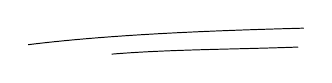
\begin{tikzpicture}[x=1cm,y=1cm]
\draw[line width=.35pt] (0,0) .. controls (1.05,.13) and (2.35,.18) .. (3.5,.21);
\draw[line width=.35pt] (1.06,-.12) .. controls (1.78,-.06) and (2.60,-.06) .. (3.43,-.03);
\end{tikzpicture}}

\margin{\unsure{11.7.|II.7.}}On va faire une \uline{\unsure{categorie|catégorie}} avec les \unsure{disjoncteurs|disponcteurs}, en prenant comme morphismes $\underline E_{\unsure{,|\ell|1}}\unsure{\longrightarrow|\mbox{---}}\underline{E'}$ les correspondances qui satisfont a) b) de la page 94 avec la composition (si $\underline E\xrightarrow{\alpha}\underline{E'}\xrightarrow{\beta}\underline{E''}$)
\[
 \beta\underset{\mathrm{dis}}{\circ}\alpha=
 \deleted{\bigl(\beta\underset{\mathrm{ens}}{\circ}\alpha}
 \operatorname{supp}_{E''}^{\bullet}\bigl(\beta\underset{\mathrm{ens}}{\circ}\alpha\bigr).
\]
\unsure{Cette|Cela}
% archive sheet number: 98
